\documentclass[11pt,a4paper]{article}
\usepackage[margin=2.15cm]{geometry}
\usepackage[T1]{fontenc}
\usepackage{lmodern,microtype}
\usepackage{amsmath,amssymb,graphicx,booktabs,tabularx,array}
\usepackage{caption,placeins,xcolor,hyperref,xurl,fancyvrb,pdflscape,needspace}
\hypersetup{colorlinks=true,linkcolor=blue!50!black,citecolor=blue!50!black,
  urlcolor=blue!50!black,pdftitle={Positive distribution-function modelling of Omega Centauri},
  pdfauthor={oCen dm project notes}}
\graphicspath{{../plots/}}
\captionsetup{font=small,labelfont=bf,skip=6pt}
\setlength{\emergencystretch}{2em}
\setlength{\parskip}{3pt}
\clubpenalty=10000
\widowpenalty=10000
\renewcommand{\topfraction}{0.92}
\renewcommand{\textfraction}{0.06}
\renewcommand{\floatpagefraction}{0.72}
\newcommand{\Msun}{\mathrm{M}_{\odot}}
\newcommand{\pc}{\,\mathrm{pc}}
\newcommand{\kms}{\,\mathrm{km\,s^{-1}}}
\newcommand{\DF}{\mathrm{DF}}
\newcommand{\kin}{\mathrm{kin}}
\newcommand{\phot}{\mathrm{phot}}
\newcommand{\dd}{\mathrm{d}}
\title{\vspace{-1cm}Positive distribution-function modelling of $\omega$ Centauri\\[4pt]
\large AGAMA infrastructure, numerical validation and first fitting pilot}
\author{oCen\_dm project notes}
\date{22 September 2026}

\begin{document}
\maketitle
\begin{abstract}
We describe a spherical stellar distribution-function (DF) modelling branch
built on AGAMA. Positive analytic action DFs, or positive mixtures of these
DFs, generate the stellar density and velocity moments in a common potential.
The stellar contribution to the potential is iterated to self-consistency;
a central point mass, Plummer remnants and a truncated dark halo may also
contribute. The same model predicts the photometric profile and 89 kinematic
measurements, preserving the selection-aware bin averages used in the Jeans
analysis. Four example equilibria pass independent projection and complete
resolution-doubling checks, with predicted dispersions changing by at most
$0.011$ observational errors. A positive mixture produces radial anisotropy
at intermediate radii and tangential anisotropy farther out. A short no-DM
pilot exercises the joint fitting workflow and reaches
$\chi^2_\kin=761.52$, but stops at its 96-evaluation budget before optimizer
convergence. These results establish a working and tested inference
infrastructure. They do not yet measure new dark-matter or black-hole
constraints. The DF guarantee applies to the stars; the remnant and dark-matter
components are presently specified as static gravitational sources.
\end{abstract}

\section{Purpose and scope}

The Jeans modelling sequence established diagnostic baselines for the
kinematic data. A Jeans solution specifies density, anisotropy and velocity
moments, but positive density and positive second moments alone do not
establish the existence of a non-negative phase-space DF. The new branch
starts with a positive stellar DF and derives those quantities together.
It therefore tests whether the observed photometry and kinematics can be
described by a realizable equilibrium within a stated family.

AGAMA supplies the action calculations, analytic DF implementation and
gravitational-potential machinery \cite{vasiliev2019,agama_manual}. Our
Python layer controls the spherical velocity integrals, the self-consistency
iteration, projection, data likelihood and run provenance. This branch is
separate from the existing \texttt{AgamaDFBackend}, which uses a restricted
\texttt{QuasiSpherical} inversion as a diagnostic. No inverted negative DF is
clipped in the new construction.

The current model is spherical, time independent and nonrotating in its even
DF. The luminous components share one stellar mass-to-light ratio. Density
and anisotropy can change together, including the unresolved central density
in the presence of a black hole. We retain the previous Jeans results as
benchmarks; this infrastructure does not certify or reweight their saved
posterior samples.

\section{Constructive stellar distribution functions}
\label{sec:df}

\subsection{Actions and the single-component family}

For a spherical potential with $\Phi(\infty)=0$, the energy and angular
momentum of a bound star are
\begin{equation}
 E=\tfrac12|\boldsymbol v|^2+\Phi(r)<0,\qquad
 L=|\boldsymbol r\times\boldsymbol v|.
\end{equation}
The radial action is
\begin{equation}
 J_r(E,L)=\frac{1}{\pi}\int_{r_{\rm peri}}^{r_{\rm apo}}
 \left[2\{E-\Phi(r)\}-\frac{L^2}{r^2}\right]^{1/2}\dd r.
 \label{eq:jr}
\end{equation}
AGAMA's action coordinates satisfy $L=J_z+|J_\phi|$ in the spherical case.
We use its \texttt{DoublePowerLaw} family, with rotation, the optional core
modifier and the optional exponential action cutoff disabled:
\begin{align}
 f_i(J_r,L)&=C_i
 \left[1+\left(\frac{J_{0,i}}{h_i}\right)^{\eta_i}\right]^{\Gamma_i/\eta_i}
 \left[1+\left(\frac{g_i}{J_{0,i}}\right)^{\eta_i}\right]^{-B_i/\eta_i},
 \label{eq:df}\\
 h_i&=h_{r,i}J_r+\frac{3-h_{r,i}}{2}L,\qquad
 g_i=g_{r,i}J_r+\frac{3-g_{r,i}}{2}L. \label{eq:actionweights}
\end{align}
Equal coefficients of $J_z$ and $|J_\phi|$ enforce spherical symmetry.
The coefficients $h_r$ and $g_r$ control relative orbital weights; they are
not values of the velocity-anisotropy parameter $\beta$.

The parameter domain is $J_0>0$, $\eta>0$, $\Gamma<3$, $B>3$ and
$0<h_r,g_r<3$. It makes equation~\eqref{eq:df} non-negative throughout bound
action space and gives finite total mass. Negative $\Gamma$ is allowed and
suppresses the DF at small actions. At the isolated zero-action limit the
DF may vanish or diverge while remaining integrable. Unbound phase space has
$f=0$. The point $r=0$ itself is excluded from numerical evaluation when the
potential contains an unsoftened point-mass singularity.

AGAMA determines $C_i$ using the requested component \texttt{mass}, so that
\begin{equation}
 (2\pi)^3\int f_i(\boldsymbol J)\,\dd^3J=M_i.
 \label{eq:massnorm}
\end{equation}
The integral uses $J_r,J_z\geq0$ and signed $J_\phi$. The library's
\texttt{norm} parameter instead sets a prefactor whose relation to total mass
depends on DF shape; it is not used here. Internal units are pc, $\Msun$,
km\,s$^{-1}$ and pc\,km\,s$^{-1}$ for actions.

\subsection{Positive mixtures and emergent anisotropy}

For $K$ components, we set $M_i=w_iM_\star$ and
\begin{equation}
 f_\star=\sum_{i=0}^{K-1} f_i,\qquad w_i>0,\qquad \sum_iw_i=1.
\end{equation}
These are basis components of the same observed stellar population. A common
mass-to-light ratio makes their mass and light fractions equal. The optimizer
can vary $a_i=\ln(w_i/w_0)$ for $i\geq1$, with $a_0=0$, and recover
\begin{equation}
 w_i=\frac{\exp(a_i)}{\sum_j\exp(a_j)}.
 \label{eq:softmax}
\end{equation}
The numerical implementation subtracts the largest $a_i$ before exponentiating.
This parameterization preserves positivity and normalization without fitting
raw fractions independently.

The density and pressures follow from the DF:
\begin{equation}
 \rho_\star=\int f_\star\dd^3v,\quad
 p_r=\int v_r^2 f_\star\dd^3v,\quad
 p_t=\frac12\int(v_\theta^2+v_\phi^2)f_\star\dd^3v,
 \qquad \beta(r)=1-\frac{p_t}{p_r}.
 \label{eq:moments}
\end{equation}
Here $p_t$ refers to one tangential component. For the nonrotating DF,
$\sigma_r^2=p_r/\rho_\star$ and $\sigma_\theta^2=\sigma_\phi^2=p_t/\rho_\star$.
Neither $\rho_\star(r)$ nor $\beta(r)$ is imposed independently. Mixtures with
different action scales and orbital weights can produce an anisotropy
turnover as their contributions to the pressure change with radius.

Figure~\ref{fig:profiles} demonstrates this flexibility for the example
configurations in Table~\ref{tab:examples}. The two-component example has
$\beta\simeq+0.14$ at 5 pc, $+0.04$ at 20 pc and $-1.0$ at 50 pc.
These are example equilibria, not inferred anisotropy profiles.

\begin{table}[htbp]
\centering\small
\caption{Fixed-parameter examples used for infrastructure validation.
All have $M_\star=2.7\times10^6\Msun$, $M_\bullet=10^4\Msun$,
$M_{\rm rem}=5\times10^5\Msun$, $a_{\rm rem}=5.3\pc$ and $D=5.43$ kpc.
Every DF has $\Gamma=0$, $B=7$, $\eta=2$ and $h_r=1.5$.
Halo examples have $r_s=30\pc$ and $r_t=1000\pc$.}
\label{tab:examples}
\begin{tabular}{lrrrrr}
\toprule
Example & $M_{\rm DM}(<100\pc)$ & $\gamma$ & $w_i$ & $J_{0,i}$ & $g_{r,i}$\\
 & [$\Msun$] & & & [pc\,km\,s$^{-1}$] &\\
\midrule
Single DF, no DM & 0 & -- & 1 & 300 & 1.0\\
Single DF, core & $2\times10^6$ & 0 & 1 & 300 & 1.0\\
Single DF, cusp & $2\times10^6$ & 1 & 1 & 300 & 1.0\\
Two DFs, no DM & 0 & -- & 0.75, 0.25 & 260, 600 & 1.1, 2.0\\
\bottomrule
\end{tabular}
\end{table}

\begin{figure}[htbp]
\centering
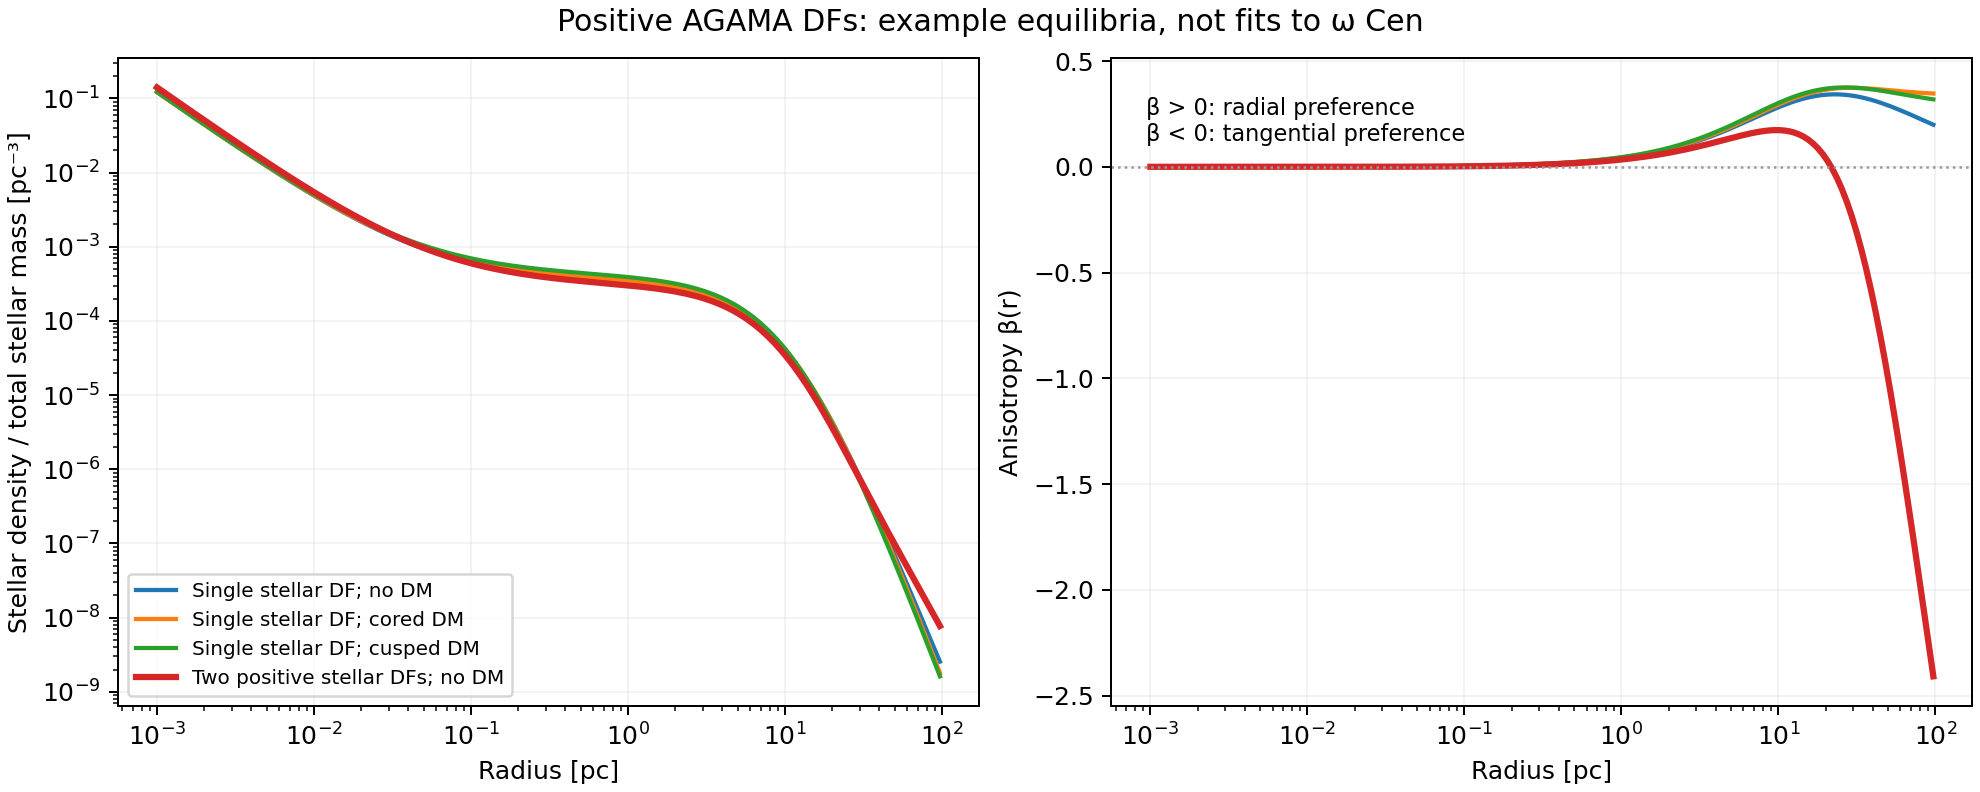
\includegraphics[width=\linewidth]{df_validation_profiles.png}
\caption{Stellar density per unit total stellar mass (left) and derived
anisotropy (right) for four positive-DF example equilibria. All use an exact
central point mass; their inner stellar density is an output of the DF.
The two-component model changes from radial preference at intermediate radii
to tangential preference farther out. The examples demonstrate realizable
profile shapes and have not been optimized against the observations.}
\label{fig:profiles}
\end{figure}
\FloatBarrier

\section{Gravitational model and self-consistency}

\subsection{Live stellar gravity and static components}

The total potential is
\begin{equation}
 \Phi=\Phi_\star[f_\star]+\Phi_\bullet+\Phi_{\rm rem}+\Phi_{\rm DM},
 \quad \Phi_\bullet=-\frac{GM_\bullet}{r},\quad
 \Phi_{\rm rem}=-\frac{GM_{\rm rem}}{\sqrt{r^2+a_{\rm rem}^2}}.
\end{equation}
AGAMA's Plummer potential with zero scale radius implements the exact point
mass; no BH softening is introduced. The optional dark halo follows the
same truncated generalized NFW law as the Jeans branch:
\begin{equation}
 \rho_{\rm DM}(r)=\rho_s
 \left(\frac r{r_s}\right)^{-\gamma}
 \left(1+\frac r{r_s}\right)^{\gamma-3}
 \left[1+\left(\frac r{r_t}\right)^2\right]^{-2}.
 \label{eq:halo}
\end{equation}
The code fixes $\rho_s$ from $M_{\rm DM}(<100\pc)$ and constructs a spherical
multipole potential. The supplied halo examples use $\gamma=0$ or 1.

Only stellar gravity responds to the DF iteration. The remnant and halo
densities are non-negative gravitational sources but have no specified DFs
in this branch. Consequently, stellar phase-space consistency is established
within the numerical tolerances, while a fully live multi-component
phase-space model remains a later extension. Positive stellar DFs also do
not, by themselves, prove dynamical stability or survival in the Galactic tide.

\subsection{Velocity quadrature and the iteration}

For an even spherical DF, let $\mu=|v_r|/v\in[0,1]$ and
$v_{\rm esc}(r)=\sqrt{-2\Phi(r)}$. We evaluate
\begin{align}
 \rho_\star(r)&=4\pi\int_0^{v_{\rm esc}}v^2\dd v\int_0^1 f_\star\dd\mu,\\
 p_r(r)&=4\pi\int_0^{v_{\rm esc}}v^4\dd v\int_0^1\mu^2 f_\star\dd\mu,\\
 p_t(r)&=2\pi\int_0^{v_{\rm esc}}v^4\dd v\int_0^1(1-\mu^2)f_\star\dd\mu.
 \label{eq:quadrature}
\end{align}
AGAMA evaluates the actions and analytic DF at each quadrature point.
Positive Gauss--Legendre weights preserve the sign of these integrals.

The iteration begins with a stellar Plummer seed of the requested stellar
mass and a 5-pc scale radius, plus the static components. At each iteration
we integrate the DF over velocities, interpolate $\ln\rho_\star$ against
$\ln r$, construct the new stellar multipole potential, and recompute the
actions in the total potential. The density interpolation uses a cubic spline
with explicit power-law continuation at both ends; unacceptable finite-mass
asymptotes are rejected. The seed is a numerical starting point, not the
stellar density retained in the final model.

Both density and total force must converge. Testing the force alone could
hide a poorly converged stellar density when a static component dominates
the potential. The default stopping criterion is
\begin{equation}
 \max_{r_j}\left\{
 \left|\frac{\rho^{(n)}_\star(r_j)}{\rho^{(n-1)}_\star(r_j)}-1\right|,
 \left|\frac{F^{(n)}(r_j)}{F^{(n-1)}(r_j)}-1\right|\right\}<5\times10^{-4},
 \label{eq:convergence}
\end{equation}
within 50 iterations. A fresh density integral in the final potential then
uses twice the velocity quadrature order at geometric midpoints between
radial grid nodes. The maximum discrepancy from the interpolated density
must be below 0.5\%, as must the error in the total stellar mass inferred
from its potential. Failure raises a numerical rejection; the code does not
replace negative or non-finite values with a floor.

An early prototype using AGAMA's standard \texttt{SelfConsistentModel} helper
showed a discrepancy of approximately 11\% near 0.008 pc between its density
representation and a fresh DF integral. Independent spherical velocity
quadrature confirmed that discrepancy. The explicit iteration above avoids
it in the tested models and exposes the integration resolution for checking.
This observation concerns the tested configuration; it is not a general
diagnosis of AGAMA or a modification to the installed library.

\begin{table}[htbp]
\centering\small
\caption{Default numerical settings. The final validation rebuild doubles all
four node counts and halves the iteration tolerance. The radial domain is
unchanged in that resolution test.}
\label{tab:numerics}
\begin{tabular}{lr}
\toprule
Quantity & Default\\
\midrule
Radial integration domain & $10^{-4}$--$10^5$ pc\\
Spherical potential/density nodes & 160\\
Velocity nodes in each of $v/v_{\rm esc}$ and $\mu$ & 64\\
Intrinsic density/pressure interpolation nodes & 240\\
Line-of-sight quadrature nodes & 128\\
Maximum iterations & 50\\
Iteration tolerance & $5\times10^{-4}$\\
Maximum density and mass closure errors & $5\times10^{-3}$\\
\bottomrule
\end{tabular}
\end{table}

\section{From the DF to the observations}

\subsection{Projection and binning}

The cached density and pressure tables are interpolated in logarithms using
shape-preserving piecewise cubic interpolation. With $q=R^2/r^2$, the
projected surface density and unnormalized second moments are
\begin{align}
 \Sigma(R)&=2\int_R^\infty\frac{\rho_\star(r)r\,\dd r}{\sqrt{r^2-R^2}},\\
 P_{\rm los}(R)&=2\int_R^\infty
 \frac{[(1-q)p_r+qp_t]r\,\dd r}{\sqrt{r^2-R^2}},\\
 P_{\rm pmR}(R)&=2\int_R^\infty
 \frac{[qp_r+(1-q)p_t]r\,\dd r}{\sqrt{r^2-R^2}},\\
 P_{\rm pmT}(R)&=2\int_R^\infty
 \frac{p_t r\,\dd r}{\sqrt{r^2-R^2}}.
 \label{eq:projection}
\end{align}
The substitution $r=R\cosh u$ removes the integrable endpoint singularity.
Numerically the upper limit is the radial integration boundary, $10^5$ pc;
requests beyond one hundredth of that radius require a wider grid. These
are projections of DF-derived moments. The Jeans equation is used as an
independent test, not as a second moment solver in this branch.

The ratio $P_k/\Sigma$ is averaged using the selection representation saved
with each observed profile. HST and Gaia component bins use equal-weight
radial quantiles of the measured stars. For profiles with annular edges and
no stored stellar quantiles, six Gauss--Legendre nodes implement the
tracer-weighted average
\begin{equation}
 \overline{v_k^2}_b=
 \frac{\int_{R_{b,-}}^{R_{b,+}}P_k(R)R\,\dd R}
      {\int_{R_{b,-}}^{R_{b,+}}\Sigma(R)R\,\dd R}.
\end{equation}
A profile without edges uses its representative radius. Proper-motion
second moments are divided by $(4.74047046D)^2$ for $D$ in kpc, giving
(mas\,yr$^{-1}$)$^2$. Angular radii become physical radii through
$R=r_{\rm arcsec}(1000D)/206264.806$.

\subsection{Streaming and the kinematic likelihood}

For continuity with the baseline data treatment, the predicted dispersion in
a bin is
\begin{equation}
 s_b=\left(\overline{v_k^2}_b-S_b\right)^{1/2},
 \label{eq:streaming}
\end{equation}
where $S_b$ is the saved published streaming variance in the corresponding
observational units. A non-positive radicand is rejected. This is a
moment-level approximation to rotation. We have not fitted the odd part of
a rotating DF, and positivity of the even DF does not establish that a
positive rotating extension can reproduce every adopted streaming moment.

The five profiles contain 21 HST radial, 21 HST tangential, 29 MUSE LOS,
nine Gaia radial and nine Gaia tangential bins. For a measured dispersion
$d_b$ with lower and upper errors $e_{b,-},e_{b,+}$, the normalized
split-normal likelihood is
\begin{equation}
 \ln\mathcal L_\kin=
 \sum_b\left[-\frac{(s_b-d_b)^2}{2e_b^2}
 +\ln\frac{\sqrt{2/\pi}}{e_{b,-}+e_{b,+}}\right],\qquad
 e_b=\begin{cases}e_{b,+},&s_b>d_b,\\e_{b,-},&s_b\leq d_b.\end{cases}
 \label{eq:likelihood}
\end{equation}
The current likelihood is diagonal. Reusing the selected profiles and their
error arrays does not establish that every bin or dataset is statistically
independent. No instrument scale factors are fitted in the supplied examples.

\subsection{Photometric shape and the joint objective}

The composite profile combines inner HST star counts and outer surface
brightness, with 82 retained points of positive relative weight. Under the
common stellar mass-to-light ratio, write
\begin{equation}
 m_j=-2.5\log_{10}\Sigma(R_j),\quad
 \widehat A=\frac{\sum_j(\mu_j-m_j)/\epsilon_j^2}
                 {\sum_j1/\epsilon_j^2},\quad
 \chi^2_\phot=\sum_j\frac{(m_j+\widehat A-\mu_j)^2}{\epsilon_j^2}.
 \label{eq:photometry}
\end{equation}
The common magnitude zero-point $\widehat A$ is profiled out; photometry
therefore constrains shape without fixing the stellar mass through an
assumed absolute mass-to-light ratio.

The composite profile provides relative weights $W_j$, not calibrated
photometric uncertainties. The pilot explicitly adopts
$\epsilon_j=0.1/\sqrt{W_j}$ mag, with zero-weight points discarded. These
errors define the diagnostic weighting and omit the covariance introduced
by the profile splice. Users may supply explicit per-point errors in a
photometric snapshot instead.

The local optimizer minimizes
\begin{equation}
 Q=\chi^2_\kin+\chi^2_\phot.
 \label{eq:objective}
\end{equation}
The normalized kinematic and profiled Gaussian photometric log-likelihoods
are also saved. The search bounds are not a complete set of inference
priors. Photometric error calibration, the zero-point treatment, distance
and mixture priors need explicit choices before computing posterior
probabilities or evidences. No DF-family evidence is reported here.

\section{Numerical validation}
\label{sec:validation}

The recorded verification pass contains 94 successful tests: 23 new DF tests
and 71 existing consistency, anisotropy and run-replay tests. The new controls
include positive-mixture normalization and spherical invariance, an analytic
isotropic Kepler DF, exact point-mass gravity, the independent Jeans moment
equation, radial integration of stellar mass, and halo normalization and force
checks. They also exercise bound and unbound phase-space evaluation, unit
protection, failed convergence, photometric normalization, bin averages and
infeasible streaming subtraction. The installed library identifies itself as
AGAMA 1.0.152, compiled on 8 June 2025.

For each full-data evaluation, we compare equation~\eqref{eq:projection} with
AGAMA's native projected \texttt{GalaxyModel.moments} calculation at 16 radii
from 0.02 to 80 pc. The maximum relative discrepancy among surface density
and all three projected pressures must be below 0.5\%. We then rebuild the
equilibrium with the refined settings in Table~\ref{tab:numerics}. For each
of the 89 kinematic bins we require
\begin{equation}
 \delta_b=\frac{|s_b^{\rm refined}-s_b^{\rm default}|}
                  {\min(e_{b,-},e_{b,+})}<0.1.
 \label{eq:refine}
\end{equation}
These checks measure numerical accuracy, separately from agreement with data.
They do not prove convergence for every possible parameter choice. Particularly
extreme DFs may need a larger domain or finer quadrature.

\begin{table}[htbp]
\centering\small
\caption{Measured validation errors. Density closure uses a fresh DF integral
at intermediate radii and doubled velocity order. Mass closure compares the
stellar potential's total mass with its requested DF mass. Projection is the
largest discrepancy from native AGAMA surface-density/pressure integrals.
The last column is the largest refined dispersion shift in data-error units.}
\label{tab:validation}
\begin{tabular}{lrrrr}
\toprule
Model & Density [\%] & Mass [\%] & Projection [\%] & $\max\delta_b$\\
\midrule
Single DF, no DM & 0.02879 & 0.000439 & 0.49196 & 0.000605\\
Single DF, core & 0.05801 & 0.000386 & 0.11473 & 0.008531\\
Single DF, cusp & 0.04631 & 0.000434 & 0.03209 & 0.000664\\
Two DFs, no DM & 0.04490 & 0.000204 & 0.05698 & 0.010868\\
No-DM pilot & 0.03578 & 0.000630 & 0.06470 & 0.008509\\
\midrule
Acceptance limit & 0.5 & 0.5 & 0.5 & 0.1\\
\bottomrule
\end{tabular}
\end{table}

All four example equilibria and the pilot pass these checks
(Figure~\ref{fig:validation}). The initial single-DF no-DM example is closest
to the native-projection tolerance, at 0.492\%; its complete resolution test
changes the binned dispersions by only 0.000605 data errors. The tests share
AGAMA's action and potential machinery, although their integration routes
differ. The analytic Kepler control adds a reference that does not depend on
the general action calculation for its expected density and pressure.

\begin{figure}[htbp]
\centering
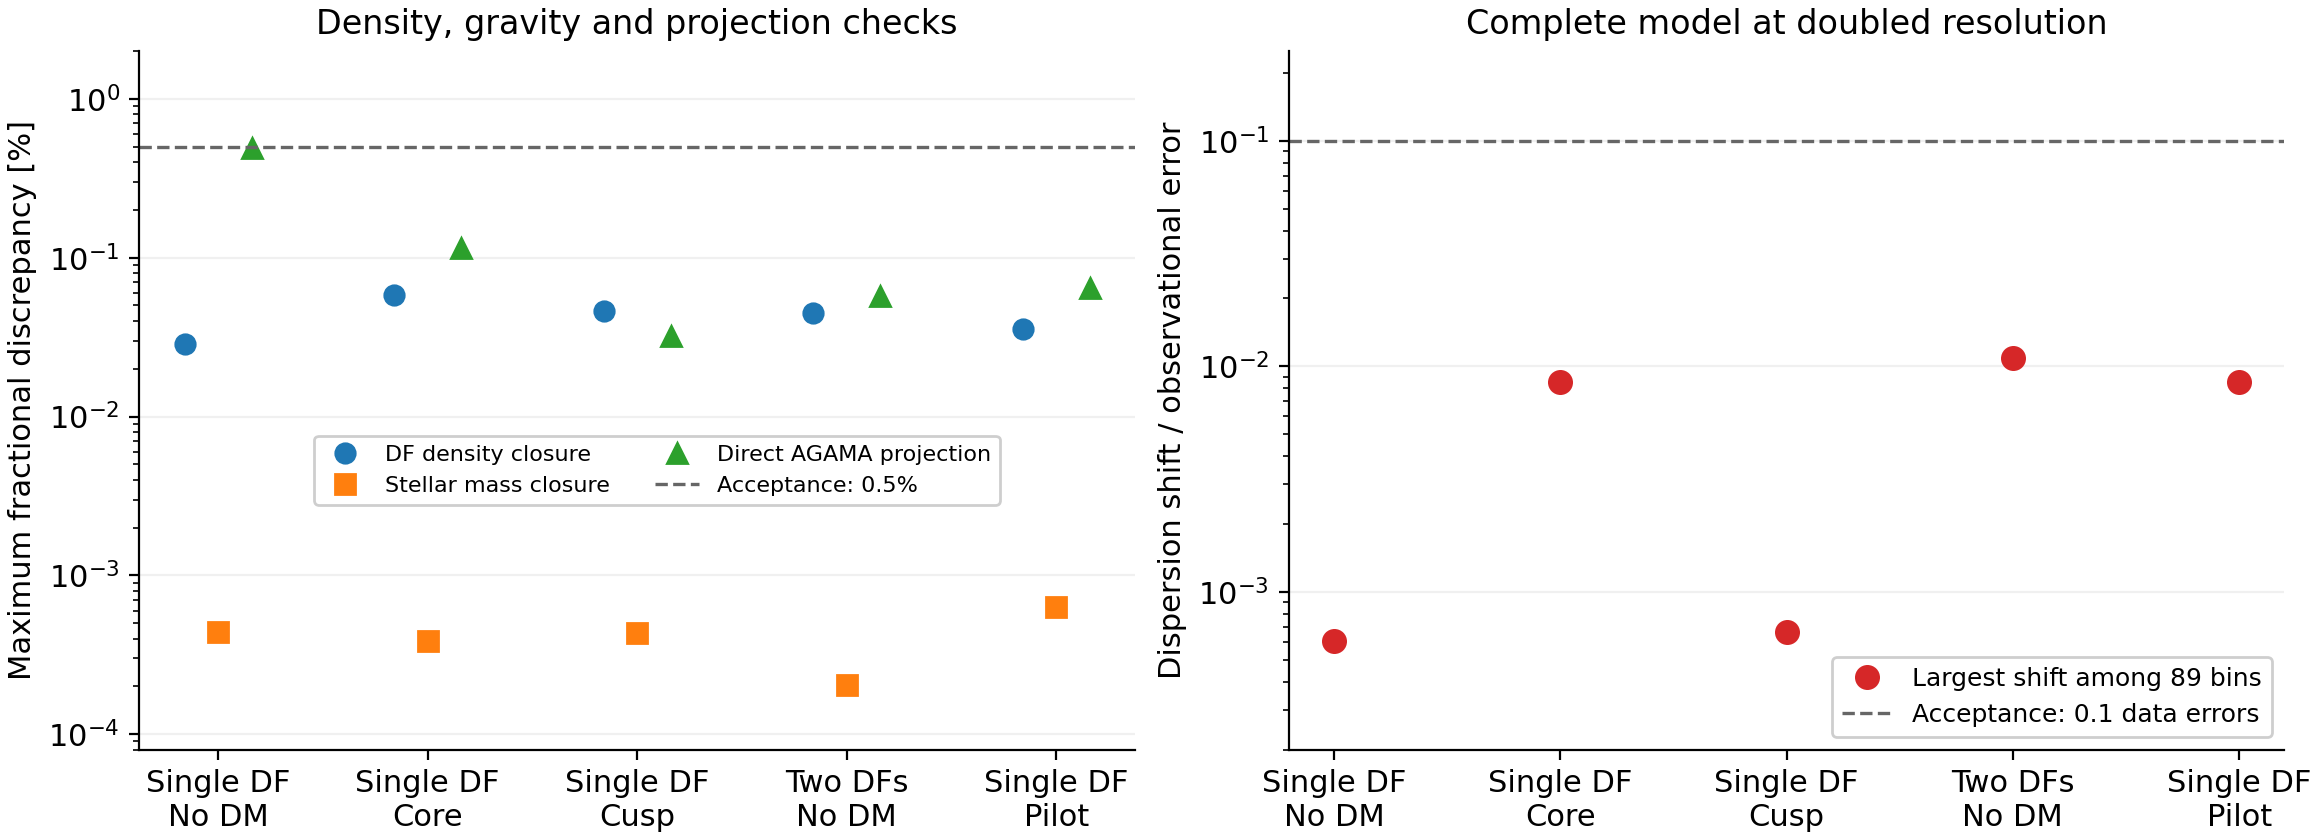
\includegraphics[width=\linewidth]{df_numerical_validation.png}
\caption{Numerical checks for the four fixed-parameter examples and the
bounded no-DM pilot. Left: maximum fractional density, mass and direct
projection discrepancies; the dashed line marks 0.5\%. Right: largest
change in a predicted dispersion when the entire calculation is rebuilt at
doubled resolution, divided by the smaller quoted error of that bin.
The dashed line marks 0.1 observational errors. Passing these tests
establishes numerical control for these configurations, not a good fit.}
\label{fig:validation}
\end{figure}
\FloatBarrier

\section{First bounded fitting pilot}
\label{sec:pilot}

The pilot starts from the single-component no-DM configuration in
Table~\ref{tab:examples}. Bounded Powell optimization varies the six
coordinates in Table~\ref{tab:pilotparams}; the remnant component, distance,
$\eta$ and $h_r$ remain fixed. The example configuration files for DM models
likewise leave the halo parameters fixed unless additional coordinates are
explicitly supplied. These evaluations are not completed no-DM/DM comparisons.

\begin{table}[htbp]
\centering\small
\caption{Search coordinates and the best joint model visited in the 96-call
no-DM pilot. Logarithmic coordinates describe the search transformation;
the intervals are optimizer bounds, not posterior priors. No uncertainties
are implied. Fixed values are $M_{\rm rem}=5\times10^5\Msun$,
$a_{\rm rem}=5.3\pc$, $D=5.43$ kpc, $\eta=2$ and $h_r=1.5$.}
\label{tab:pilotparams}
\begin{tabular}{llrr}
\toprule
Parameter & Coordinate & Search interval & Pilot value\\
\midrule
$M_\star$ [$\Msun$] & $\ln M_\star$ & $10^6$--$6\times10^6$ & $3.13958\times10^6$\\
$J_0$ [pc\,km\,s$^{-1}$] & $\ln J_0$ & 80--1000 & 293.094\\
$B$ & Linear & 4.5--10 & 6.99359\\
$g_r$ & Linear & 0.5--2.4 & 1.16588\\
$\Gamma$ & Linear & $-2$--1.5 & 0.163119\\
$M_\bullet$ [$\Msun$] & $\ln M_\bullet$ & $10^2$--$10^5$ & 12356.2\\
\bottomrule
\end{tabular}
\end{table}

After 96 objective evaluations, the best joint objective falls from
17\,972.67 to 1423.82. Its kinematic contribution falls from 15\,881.77 to
761.52, and its photometric contribution from 2090.90 to 662.30.
The recorded elapsed time is 294 s, including validation and report generation.
The history contains two numerically rejected trials. Figure~\ref{fig:optimization}
shows the accepted objective values and the best joint model retained after
each call. The separate contributions need not decrease on every improvement
in their sum.

\textbf{The optimizer reached its evaluation limit before convergence.}
The residuals in Figure~\ref{fig:pilot} remain substantial, particularly in
the inner HST and photometric profiles. Table~\ref{tab:fit} gives the
contributions to the kinematic objective. This pilot validates the fitting
workflow; it does not measure the fit penalty imposed by DF positivity,
establish the best attainable fit of the family, or yield a new BH or DM
constraint. We do not assign a reduced chi-squared interpretation to the joint
objective with these adopted photometric errors.

\begin{figure}[htbp]
\centering
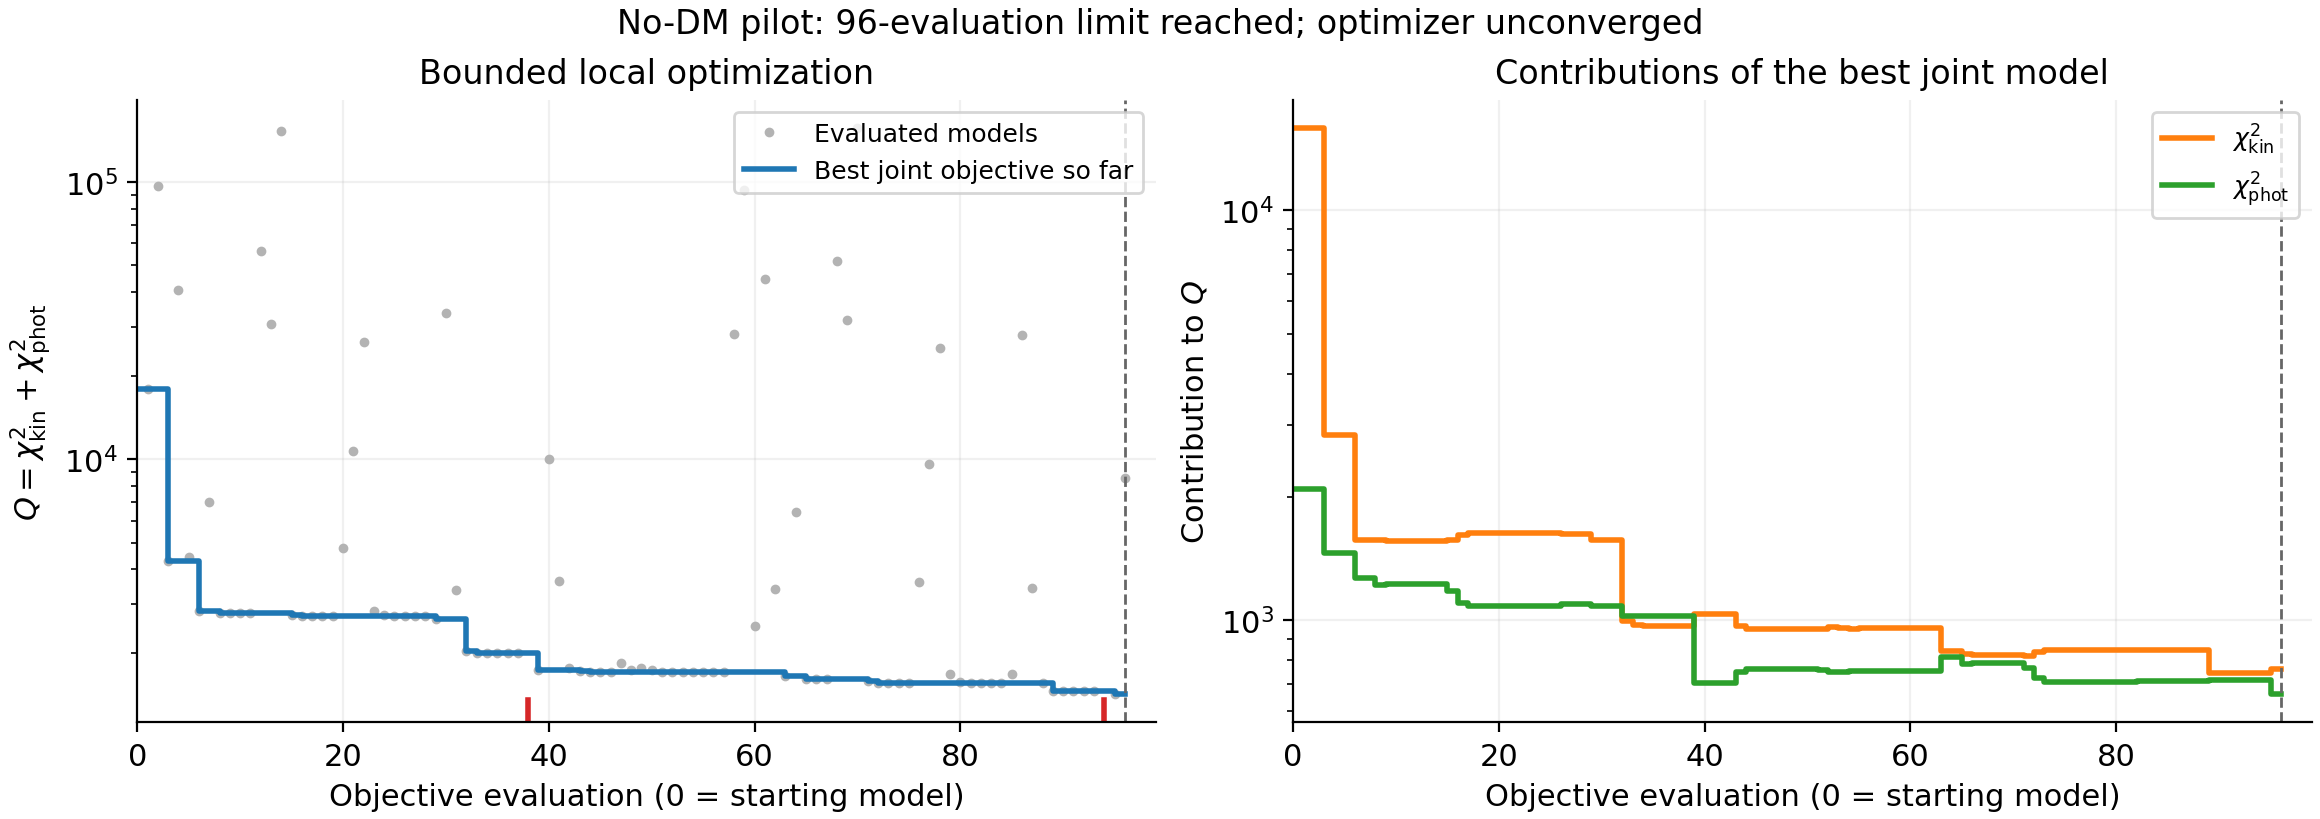
\includegraphics[width=\linewidth]{df_pilot_optimization.png}
\caption{Recorded progress of the bounded no-DM pilot. Left: grey points are
finite objective evaluations and the blue step curve is the lowest joint
objective visited so far. Short red ticks at the bottom mark rejected
numerical trials. Right: kinematic and photometric contributions of that
same best joint model, rather than independent minima of each term.
The vertical dashed line marks the imposed 96-call limit. The optimizer has
not converged.}
\label{fig:optimization}
\end{figure}

\begin{table}[htbp]
\centering\small
\caption{Objective contributions for the best joint model visited by the pilot.}
\label{tab:fit}
\begin{tabular}{lrr}
\toprule
Profile & Number of bins & $\chi^2$ contribution\\
\midrule
HST radial PM & 21 & 313.09\\
HST tangential PM & 21 & 281.63\\
MUSE LOS & 29 & 90.15\\
Gaia radial PM & 9 & 58.98\\
Gaia tangential PM & 9 & 17.67\\
\midrule
Kinematic total & 89 & 761.52\\
Photometric shape (one profiled zero-point) & 82 & 662.30\\
Joint objective & & 1423.82\\
\bottomrule
\end{tabular}
\end{table}

\begin{landscape}
\begin{figure}[p]
\centering
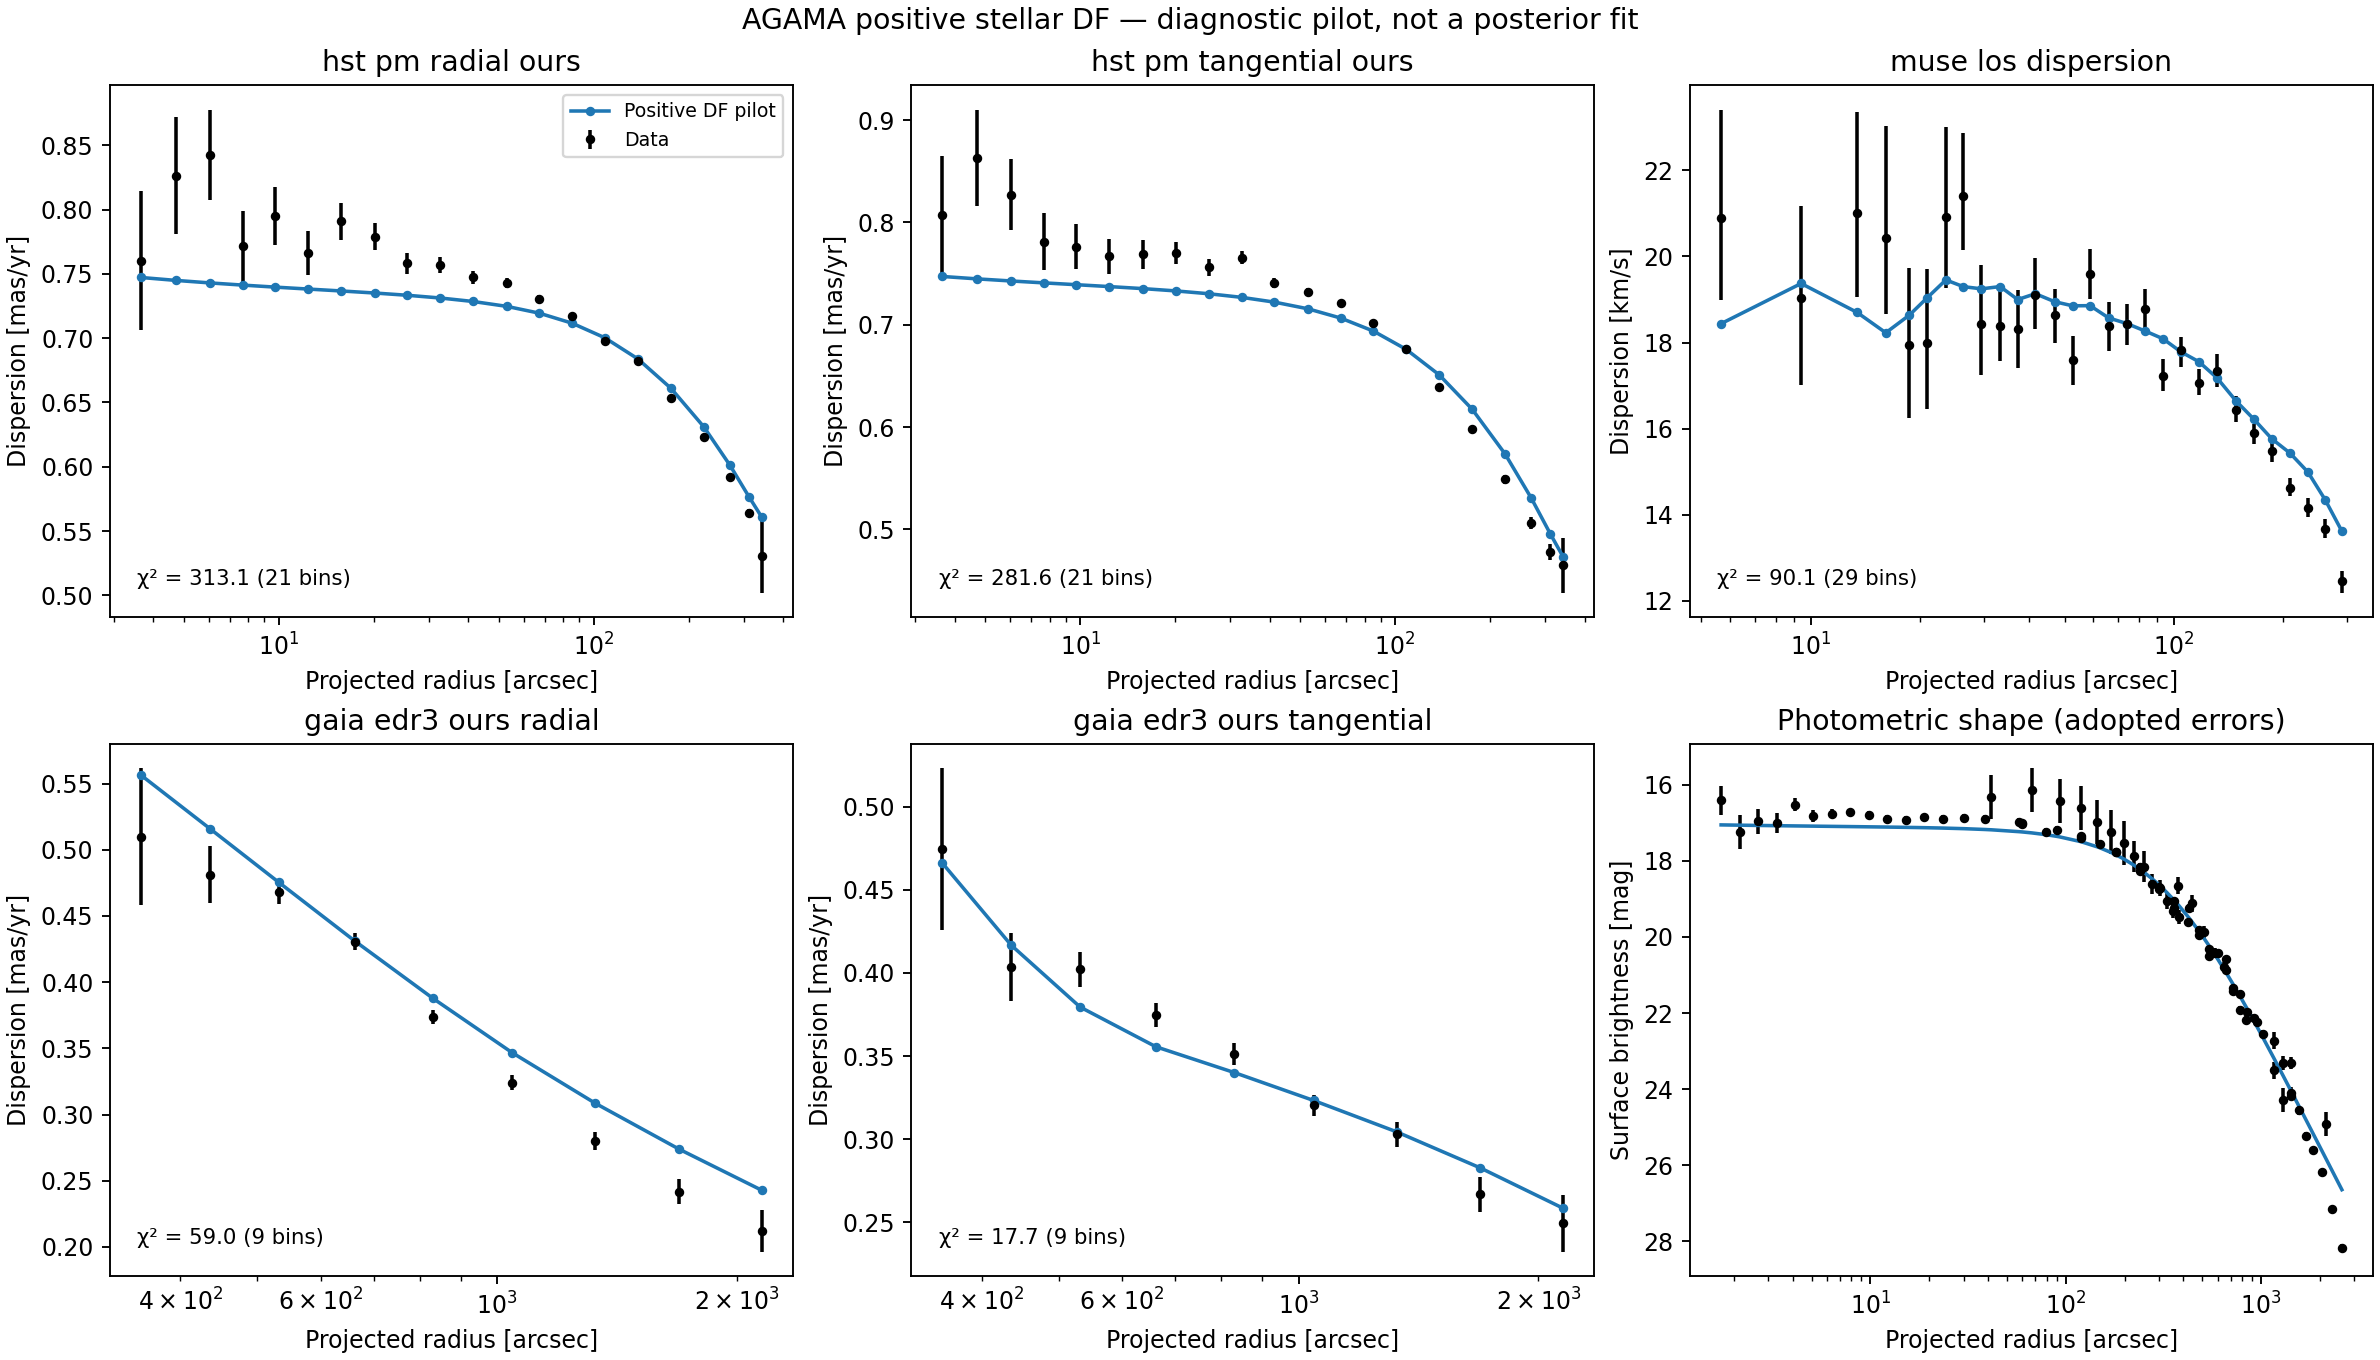
\includegraphics[width=\linewidth]{df_pilot_no_dm_20260922.png}
\caption{The bounded no-DM pilot against all five kinematic profiles and
the composite photometric profile. Model points use each observed bin's
selection-aware second-moment average and saved streaming correction.
The lines connect these bin predictions; they are not a continuously
sampled intrinsic velocity-dispersion profile. Photometric bars show the
adopted diagnostic errors, $0.1/\sqrt{W_j}$ mag. The common photometric
zero-point is fitted. The clear remaining residuals require further
optimization and model comparisons.}
\label{fig:pilot}
\end{figure}
\end{landscape}
\FloatBarrier

The pilot's refined equilibrium changes its kinematic objective to 761.41
and its joint objective to 1423.76. Its largest dispersion shift is only
0.00851 data errors, so increasing numerical resolution does not remove
the observed residuals. An independent fresh-process replay reproduces
the saved objective, all 89 predictions and the photometric prediction
exactly from the saved model and data.

\section{Software interface, records and reproduction}

\begin{table}[htbp]
\centering\small
\caption{Main interfaces in the new branch. Both source modules reside in
\texttt{src/ocen\_dm/kinematics/}.}
\label{tab:software}
\begin{tabularx}{\linewidth}{lX}
\toprule
File or interface & Responsibility\\
\midrule
\texttt{positive\_df.py} & Validated component/configuration objects, positive DFs,
  self-consistent gravity, phase-space evaluation and moment projections.\\
\texttt{df\_fit.py} & Explicit photometric data/errors, joint objective, bounded
  search coordinates and positive mixture-weight transformations.\\
\texttt{bin/run\_df\_pilot.py} & Fixed-parameter evaluation or bounded local
  optimization, snapshots, numerical refinement and a data/model figure.\\
\texttt{tests/test\_positive\_df.py} & Physical, numerical and data-interface controls.\\
\texttt{configs/df/} & Single no-DM/core/cusp and two-component examples.\\
\bottomrule
\end{tabularx}
\end{table}

The driver reads the saved kinematic snapshot and verifies its checksum and
data fingerprint. Each new run records the actual likelihood arrays,
photometric errors, configuration, source hashes and selected source copies,
evaluation history, best model, numerical diagnostics and status. Current
driver records also contain the AGAMA version and extension-binary hash.
The two-component search can vary the log mixture ratio, both action scales
and orbital weights. AGAMA units are global: the wrapper initializes the
project units once and rejects an incompatible existing unit system rather
than silently changing units of objects already in memory.

A fresh output directory is required. From the project root, with the
project environment active and AGAMA installed, a bounded pilot is:
\begin{Verbatim}[fontsize=\small,frame=single]
python bin/run_df_pilot.py \
  --config configs/df/no_dm.json \
  --out results/df/my_no_dm_pilot \
  --sigma-mag 0.1 \
  --max-evaluations 96
\end{Verbatim}
Omitting \texttt{--max-evaluations} performs a fixed-parameter evaluation
and the numerical checks. For data replay, use the options
\texttt{--data-run} with the previous run directory and
\texttt{--photometry-snapshot} with its \texttt{photometry.json} file.
For model replay, place the saved \texttt{best\_model.json} content under
the \texttt{model} key in a driver configuration and omit optimization.
The driver does not launch posterior sampling.

The records used in this note are under
\path{results/df/validation_*_20260922/},
\path{results/df/pilot_no_dm_20260922/} and
\path{results/df/replay_no_dm_20260922/}. The test and replay record is
\path{results/diagnostics/df_validation/verification.json}.
Figures~\ref{fig:validation} and~\ref{fig:optimization} are reproduced by
\path{bin/plot_df_writeup.py}, which reads saved results and launches no fits.
Its input checksums and plotted arrays are in
\path{results/plot_data/df_writeup_diagnostics.json}.

All figure exports are PNGs in \texttt{plots/}. Numerical tables and provenance
remain outside that directory. This PDF and its LaTeX source both reside in
\texttt{docs/}; build intermediates belong in
\path{results/diagnostics/df_writeup/}.

\Needspace{10\baselineskip}
\section{Next modelling steps}

The next experiment is a converged search from several starting points for
single and mixed stellar DFs, followed by matched no-DM, core and cusp
comparisons with the same photometric treatment. Varying the photometric
error scale will show how the current weighting influences the inferred
stellar density and orbital structure. The stellar/remnant mass split,
distance treatment and mixture priors need to be specified before launching
production posterior fits.

A later rotation model should fit an admissible odd DF contribution and
mean velocities jointly, replacing the present streaming approximation.
Axisymmetric structure, population-dependent tracer selections and stellar
mass segregation are further model extensions. Assigning DFs to the
remnants and DM would allow a fully live equilibrium and controlled
$N$-body realizations. Those additions would connect the mass modelling
more directly to the independent tidal-survival experiments. The present
infrastructure establishes the constructive stellar DF and numerical
controls needed for that progression.

\begin{thebibliography}{9}
\bibitem{vasiliev2019}
Vasiliev, E. 2019, \emph{AGAMA: Action-based galaxy modelling architecture},
MNRAS, 482, 1525.
\href{https://doi.org/10.1093/mnras/sty2672}{doi:10.1093/mnras/sty2672};
\href{https://arxiv.org/abs/1802.08239}{arXiv:1802.08239}.
\bibitem{agama_manual}
AGAMA reference manual, sections on spheroidal action DFs, moments and
self-consistent models. Parameter conventions checked against the locally
installed source and the
\href{https://github.com/GalacticDynamics-Oxford/Agama/blob/master/doc/reference.tex}{public manual source}.
\end{thebibliography}
\end{document}
